%%%%%%%%%%%%%%%%%%%%%%%%%%%%%%%%%%%%%%%%%%%%%%%%%%%%%%%%%%%%%%%
%% OXFORD THESIS TEMPLATE

% Use this template to produce a standard thesis that meets the Oxford University requirements for DPhil submission
%
% Originally by Keith A. Gillow (gillow@maths.ox.ac.uk), 1997
% Modified by Sam Evans (sam@samuelevansresearch.org), 2007
% Modified by John McManigle (john@oxfordechoes.com), 2015
% Modified by Ulrik Lyngs (ulrik.lyngs@cs.ox.ac.uk), 2018, for use with R Markdown
%
% Ulrik Lyngs, 25 Nov 2018: Following John McManigle, broad permissions are granted to use, modify, and distribute this software
% as specified in the MIT License included in this distribution's LICENSE file.
%
% John tried to comment this file extensively, so read through it to see how to use the various options.  Remember
% that in LaTeX, any line starting with a % is NOT executed.  Several places below, you have a choice of which line to use
% out of multiple options (eg draft vs final, for PDF vs for binding, etc.)  When you pick one, add a % to the beginning of
% the lines you don't want.


%%%%% CHOOSE PAGE LAYOUT
% The most common choices should be below.  You can also do other things, like replacing "a4paper" with "letterpaper", etc.

% This one will format for two-sided binding (ie left and right pages have mirror margins; blank pages inserted where needed):
%\documentclass[a4paper,twoside]{templates/ociamthesis}
% This one will format for one-sided binding (ie left margin > right margin; no extra blank pages):
%\documentclass[a4paper]{ociamthesis}
% This one will format for PDF output (ie equal margins, no extra blank pages):
%\documentclass[a4paper,nobind]{templates/ociamthesis}
%UL 2 Dec 2018: pass this in from YAML
\documentclass[a4paper, twoside]{templates/ociamthesis}

% add hyperref package with options from YAML %
\usepackage[colorlinks=false,pdfpagelabels,hidelinks]{hyperref}

% add float package to allow manual control of figure positioning %
% this was taken from the stackoverflow answer at: https://stackoverflow.com/a/33801326/14802285 %
\usepackage{float}
\let\origfigure\figure
\let\endorigfigure\endfigure
\renewenvironment{figure}[1][2] {
    \expandafter\origfigure\expandafter[H]
} {
    \endorigfigure
}

%UL set section header spacing
\usepackage{titlesec}
\titleformat{\chapter}
  {\normalfont\Large\bfseries}{\thechapter}{1em}{}
\titlespacing*{\chapter}{0pt}{3.5ex plus 1ex minus .2ex}{2.3ex plus .2ex}
% 
\titlespacing\subsubsection{0pt}{24pt plus 4pt minus 2pt}{0pt plus 2pt minus 2pt}

% UL 30 Nov 2018 pandoc puts lists in 'tightlist' command when no space between bullet points in Rmd file
\providecommand{\tightlist}{%
  \setlength{\itemsep}{0pt}\setlength{\parskip}{0pt}}
 
% UL 1 Dec 2018, fix to include code in shaded environments

%UL set whitespace around verbatim environments
\usepackage{etoolbox}
\makeatletter
\preto{\@verbatim}{\topsep=0pt \partopsep=0pt }
\makeatother

%UL 26 Mar 2019, enable strikethrough
\usepackage[normalem]{ulem}

%UL use soul package for correction highlighting
\usepackage{color, soul}
\usepackage{xcolor}
\definecolor{correctioncolor}{HTML}{CCCCFF}
\sethlcolor{correctioncolor}
\newcommand{\ctext}[3][RGB]{%
  \begingroup
  \definecolor{hlcolor}{#1}{#2}\sethlcolor{hlcolor}%
  \hl{#3}%
  \endgroup
}
\soulregister\ref7
\soulregister\cite7
\soulregister\autocite7
\soulregister\textcite7
\soulregister\pageref7

% user-included things with header_includes or in_header will appear here
% kableExtra packages will appear here if you use library(kableExtra)
\usepackage{booktabs}
\usepackage{longtable}
\usepackage{array}
\usepackage{multirow}
\usepackage{wrapfig}
\usepackage{float}
\usepackage{colortbl}
\usepackage{pdflscape}
\usepackage{tabu}
\usepackage{threeparttable}
\usepackage{threeparttablex}
\usepackage[normalem]{ulem}
\usepackage{makecell}
\usepackage{xcolor}


%%%%%%% PAGE HEADERS AND FOOTERS %%%%%%%%%
\usepackage{fancyhdr}
\setlength{\headheight}{15pt}
\fancyhf{} % clear the header and footers
\pagestyle{fancy}
\renewcommand{\chaptermark}[1]{\markboth{\thechapter. #1}{\thechapter. #1}}
\renewcommand{\sectionmark}[1]{\markright{\thesection. #1}} 
\renewcommand{\headrulewidth}{0pt}

\fancyhead[LO]{\emph{\leftmark}} 
\fancyhead[RE]{\emph{\rightmark}} 

% UL page number position 
\fancyfoot[C]{\emph{\thepage}} %regular pages
\fancypagestyle{plain}{\fancyhf{}\fancyfoot[C]{\emph{\thepage}}} %chapter pages

% JEM fix header on cleared pages for openright
\def\cleardoublepage{\clearpage\if@twoside \ifodd\c@page\else
   \hbox{}
   \fancyfoot[C]{}
   \newpage
   \if@twocolumn\hbox{}\newpage
   \fi
   \fancyhead[LO]{\emph{\leftmark}} 
   \fancyhead[RE]{\emph{\rightmark}} 
   \fi\fi}


%%%%% SELECT YOUR DRAFT OPTIONS
% This adds a "DRAFT" footer to every normal page.  (The first page of each chapter is not a "normal" page.)

% This highlights (in blue) corrections marked with (for words) \mccorrect{blah} or (for whole
% paragraphs) \begin{mccorrection} . . . \end{mccorrection}.  This can be useful for sending a PDF of
% your corrected thesis to your examiners for review.  Turn it off, and the blue disappears.
\correctionstrue

% IP feb 2021: option to include line numbers in PDF

%%%%% BIBLIOGRAPHY SETUP
% Note that your bibliography will require some tweaking depending on your department, preferred format, etc.
% If you've not used LaTeX before, I recommend reading a little about biblatex/biber and getting started with it.
% If you're already a LaTeX pro and are used to natbib or something, modify as necessary.
% Either way, you'll have to choose and configure an appropriate bibliography format...



\usepackage{natbib}
\setcitestyle{authoryear}
\bibliographystyle{templates/myplainnat.bst}
\addto\captionsenglish{%
  \renewcommand{\bibname}{References}
}

% This makes the bibliography left-aligned (not 'justified') and slightly smaller font.
\renewcommand*{\bibfont}{\raggedright\small}


% Uncomment this if you want equation numbers per section (2.3.12), instead of per chapter (2.18):
%\numberwithin{equation}{subsection}


%%%%% THESIS / TITLE PAGE INFORMATION
% Everybody needs to complete the following:
\title{\texttt{Research\ Project}:\\
Retrieval of plant biophysical and biochemical variables from remote sensing data using a hybrid machine learning method}
\author{Zavud Baghirov}
\college{Environmental Sciences}

% Master's candidates who require the alternate title page (with candidate number and word count)
% must also un-comment and complete the following three lines:

% Uncomment the following line if your degree also includes exams (eg most masters):
%\renewcommand{\submittedtext}{Submitted in partial completion of the}
% Your full degree name.  (But remember that DPhils aren't "in" anything.  They're just DPhils.)
\degree{}
% Term and year of submission, or date if your board requires (eg most masters)
\degreedate{Summer Semester 2021}


%%%%% YOUR OWN PERSONAL MACROS
% This is a good place to dump your own LaTeX macros as they come up.

% To make text superscripts shortcuts
	\renewcommand{\th}{\textsuperscript{th}} % ex: I won 4\th place
	\newcommand{\nd}{\textsuperscript{nd}}
	\renewcommand{\st}{\textsuperscript{st}}
	\newcommand{\rd}{\textsuperscript{rd}}

%%%%% THE ACTUAL DOCUMENT STARTS HERE
\begin{document}

%%%%% CHOOSE YOUR LINE SPACING HERE
% This is the official option.  Use it for your submission copy and library copy:
\setlength{\textbaselineskip}{22pt plus2pt}
% This is closer spacing (about 1.5-spaced) that you might prefer for your personal copies:
%\setlength{\textbaselineskip}{18pt plus2pt minus1pt}

% You can set the spacing here for the roman-numbered pages (acknowledgements, table of contents, etc.)
\setlength{\frontmatterbaselineskip}{17pt plus1pt minus1pt}

% UL: You can set the line and paragraph spacing here for the separate abstract page to be handed in to Examination schools
\setlength{\abstractseparatelineskip}{13pt plus1pt minus1pt}
\setlength{\abstractseparateparskip}{0pt plus 1pt}

% UL: You can set the general paragraph spacing here - I've set it to 2pt (was 0) so
% it's less claustrophobic
\setlength{\parskip}{2pt plus 1pt}

%
% Oxford University logo on title page
%
\def\crest{{
\includegraphics{templates/uni-logo.png}}}
\renewcommand{\university}{University of Trier}
\renewcommand{\submittedtext}{}


% Leave this line alone; it gets things started for the real document.
\setlength{\baselineskip}{\textbaselineskip}


%%%%% CHOOSE YOUR SECTION NUMBERING DEPTH HERE
% You have two choices.  First, how far down are sections numbered?  (Below that, they're named but
% don't get numbers.)  Second, what level of section appears in the table of contents?  These don't have
% to match: you can have numbered sections that don't show up in the ToC, or unnumbered sections that
% do.  Throughout, 0 = chapter; 1 = section; 2 = subsection; 3 = subsubsection, 4 = paragraph...

% The level that gets a number:
\setcounter{secnumdepth}{1}
% The level that shows up in the ToC:
\setcounter{tocdepth}{1}


%%%%% ABSTRACT SEPARATE
% This is used to create the separate, one-page abstract that you are required to hand into the Exam
% Schools.  You can comment it out to generate a PDF for printing or whatnot.

% JEM: Pages are roman numbered from here, though page numbers are invisible until ToC.  This is in
% keeping with most typesetting conventions.
\begin{romanpages}

% Title page is created here
\maketitle

%%%%% DEDICATION -- If you'd like one, un-comment the following.

%%%%% ACKNOWLEDGEMENTS -- Nothing to do here except comment out if you don't want it.


%%%%% ABSTRACT -- Nothing to do here except comment out if you don't want it.
\begin{abstract}
	This will be the abstract at the end {[}TO BE UPDATED{]}
\end{abstract}

%%%%% MINI TABLES
% This lays the groundwork for per-chapter, mini tables of contents.  Comment the following line
% (and remove \minitoc from the chapter files) if you don't want this.  Un-comment either of the
% next two lines if you want a per-chapter list of figures or tables.

% This aligns the bottom of the text of each page.  It generally makes things look better.
\flushbottom

% This is where the whole-document ToC appears:
\tableofcontents

\listoffigures
	\mtcaddchapter
  	% \mtcaddchapter is needed when adding a non-chapter (but chapter-like) entity to avoid confusing minitoc

% Uncomment to generate a list of tables:
\listoftables
  \mtcaddchapter
%%%%% LIST OF ABBREVIATIONS
% This example includes a list of abbreviations.  Look at text/abbreviations.tex to see how that file is
% formatted.  The template can handle any kind of list though, so this might be a good place for a
% glossary, etc.
% First parameter can be changed eg to "Glossary" or something.
% Second parameter is the max length of bold terms.
\begin{mclistof}{List of Abbreviations}{3.2cm}

\item[3D] Three-dimensional
\item[INFORM] Invertable Forest Reflectance Model
\item[RTM] Radiative Transfer Model
\item[SAIL] Scattering by Arbitrary Inclined Leaves
\item[PROSAIL] The combination of PROSPECT and SAIL models
\item[FLIM] Forest Light Interaction Model
\item[LAI] Leaf Area Index
\item[MLRA] Machine Learning Regression Algorithms
\item[ML] Machine Learning
\item[DT] Decision Trees
\item[ANN] Artificial Neural Networks
\item[KBMLRM] Kernel-Based Machine Learning Regression Methods
\item[RF] Random Forest
\item[RFR] Random Forest Regression
\item[LUT] Look-Up-Table
\item[NN] Neural Networks
\item[SVR] Support Vector Regression
\item[SVM] Support Vector Machines
\item[GPR] Gaussian Process Regression
\item[GP] Gaussian Process
\item[VI] Vegetation Index
\item[DR] Dimensionality Reduction
\item[WT] Wavelet Tranform
\item[PCA] Principal Component Analysis
\item[AL] Active Learning

\end{mclistof} 


% The Roman pages, like the Roman Empire, must come to its inevitable close.
\end{romanpages}

%%%%% CHAPTERS
% Add or remove any chapters you'd like here, by file name (excluding '.tex'):
\flushbottom

% all your chapters and appendices will appear here
\hypertarget{methods}{%
\chapter{Methods}\label{methods}}

This section explains the methods used in this research.

\hypertarget{local-sensitivity-analysis}{%
\section{Local sensitivity analysis}\label{local-sensitivity-analysis}}

Local sensitivity analysis was performed to assess the effect of each of the main 6 plant biochemical and biophysical variables on the PRISMA image bands. In the local sensitivity analysis simulation is performed by keeping all the variables constant at their determined fixed or default values except the parameter of interest. This way the effect of a specific parameter on the simulated spectra can be assessed. In this research the plant parameters \(C_{ab}\), \(C_{w}\), \(C_{m}\), \(LAI_{s}\), \(CD\) and \(SD\) were varied each 15 times (Table (\ref{tab:tsvaried})), while keeping the rest of the variables at their default values (Table (\ref{tab:tsfixed})). The default and varied values were chosen based on the literature (e.g. \citet{darvishzadeh2019mapping}; \citet{laurent2011inversion}; \citet{schlerf2012vegetation}) where similar RTM method used to simulate reflectance for Spruce trees.

Table \ref{tab:tsvaried} shows the 6 parameters that were varied, their units, minimum and maximum values. Each parameter was varied 15 times, meaning 15 different spectra were simulated for each variable.

\begin{table}[H]

\caption{\label{tab:tsvaried}INFORM Parameters varied in local sensitivity analysis (each parameter were varied 15 times)}
\centering
\begin{tabu} to \linewidth {>{\raggedright\arraybackslash}p{8cm}>{\raggedright}X>{\raggedright}X>{\raggedright}X>{\raggedright}X}
\toprule
Parameter & Abbrev. & Unit & Min & Max\\
\midrule
Chlorophyll content & $C_{ab}$ & $\frac{\mu g}{cm^2}$ & 20 & 60\\
Equivalent water thickness & $C_{w}$ & $\frac{g}{cm^2}$ & 0.0035 & 0.035\\
Leaf dry matter content & $C_{m}$ & $\frac{g}{cm^2}$ & 0.008 & 0.03\\
Leaf area index (single) & $LAI_{s}$ & $\frac{m^2}{m^2}$ & 0 & 7\\
Stem density & $SD$ & $ha^{-1}$ & 200 & 5000\\
\addlinespace
Crown diameter & $CD$ & $m$ & 1.5 & 8.5\\
\bottomrule
\end{tabu}
\end{table}

\newpage

Table \ref{tab:tsfixed} shows the determined default values for each INFORM parameter that were kept during the sensitivity simulation while one of the parameter was varied (Table \ref{tab:tsvaried}).

\begin{table}[H]

\caption{\label{tab:tsfixed}INFORM Parameters that were kept constant while one parameter was varied at a time}
\centering
\begin{tabu} to \linewidth {>{\raggedright\arraybackslash}p{8cm}>{\raggedright}X>{\raggedright}X>{\raggedright}X}
\toprule
Parameter & Abbr & Unit & Value\\
\midrule
Leaf structure parameter & $N$ & $-$ & 3\\
Chlorophyll content & $C_{ab}$ & $\frac{\mu g}{cm^2}$ & 40\\
Leaf cartenoid content & $C_{ar}$ & $\frac{\mu g}{cm^2}$ & 8\\
Brown Pigment Content & $C_{brown}$ & $-$ & 0.001\\
Equivalent water thickness & $C_{w}$ & $\frac{g}{cm^2}$ & 0.0117\\
\addlinespace
Leaf dry matter content & $C_{m}$ & $\frac{g}{cm^2}$ & 0.03\\
Average leaf inclination angle & $ALIA$ & $^{\circ}$ & 65\\
Leaf area index (single) & $LAI_{s}$ & $\frac{m^2}{m^2}$ & 6\\
Leaf area index (understorey) & $LAI_{u}$ & $\frac{m^2}{m^2}$ & 0.5\\
Hot spot parameter & $Hot$ & $\frac{m}{m}$ & 0.02\\
\addlinespace
Solar zenith angle & $tts$ & $^{\circ}$ & 45.43\\
Observer zenith angle & $tto$ & $^{\circ}$ & 0\\
Sun-sensor azimuth angle & $psi$ & $^{\circ}$ & 181.41\\
Soil brightness & $\alpha_{soil}$ & $-$ & 0.5\\
Stem density & $SD$ & $ha^{-1}$ & 700\\
\addlinespace
Crown diameter & $CD$ & $m$ & 5\\
Mean Height & $H$ & $m$ & 20\\
Fraction of diffuse incoming & $skyl$ & $-$ & 0.1\\
Soil reflectance spectrum & $B_{g}$ & $-$ & default\\
\bottomrule
\end{tabu}
\end{table}

\emph{Solar zenith angle} and \emph{Sun-sensor azimuth angle} were calculated based on the PRISMA image acquisition parameters (date, lat/long etc.) using the \emph{solar position calculator} at \url{https://www.esrl.noaa.gov/gmd/grad/solcalc/azel.html}.

RTM models PROSPECT5, 4SAIL and FLIM were coupled (INFORM) in order to simulate canopy reflectance. Simulations were carried out using the \emph{ccrtm} package \citep{ccrtm} in \emph{R} \citep{r}. The default soil spectra provided by the the \emph{ccrtm} package \citep{ccrtm} was used for the simulations. Spectral resampling was performed in order to resample the INFORM output spectra (1nm resolution) into PRISMA image bands. For spectral resampling the \emph{R} package \emph{hsdar} \citep{hsdar} was utilized.

\hypertarget{rtm-simulation-inform}{%
\section{RTM simulation (INFORM)}\label{rtm-simulation-inform}}

PROSPECT5, 4SAIL and FLIM RTM models were coupled (INFORM) to simulate forest canopy reflectance based on different values of plant biophysical and biochemical parameters. The 6 parameters that were mentioned in the previous chapter were varied and spectra was simulated based on each combination of these variables. The number of combinations increase exponentially, which in turn requires increased computational power. Therefore, the trade-off must be taken into account between computational power or time and accurate simulation.

Different authors suggest different number of LUT size for RTM simulation. For example, \citet{danner2021efficient} mention that LUT size of minimum 50,000 is recommended. \citet{ali2020machine} and \citet{darvishzadeh2019mapping} created a LUT size of 100,000 and 500,000 respectively.

In this research, LUT size of 316,800 was created based on each combination of different plant biophysical and biochemical parameters. The range of the varied parameters and parameters that were kept constant were determined based on the suggestions of the studies that were mentioned in the previous chapter. These studies used similar methods to simulate canopy reflectance for mainly Spruce forests/trees.

Table \ref{tab:tinformfull} shows the variables that were used to simulate forest canopy parameters. Table \ref{tab:tinformfull} also contains information about the range of the values and how many times each parameter was varied.

\newpage

\begin{table}[H]

\caption{\label{tab:tinformfull}Range of full input parameters that were used to create a LUT size of 316800}
\centering
\begin{tabu} to \linewidth {>{\raggedright\arraybackslash}p{8cm}>{\raggedright}X>{\raggedright}X>{\raggedright}X>{\raggedright}X>{\raggedright}X}
\toprule
Parameter & Abbr & Unit & Min & Max & Steps\\
\midrule
Leaf structure parameter & $N$ & $-$ & 3 & 3 & $-$\\
Chlorophyll content & $C_{ab}$ & $\frac{\mu g}{cm^2}$ & 20 & 60 & 15\\
Leaf cartenoid content & $C_{ar}$ & $\frac{\mu g}{cm^2}$ & 8 & 8 & $-$\\
Brown Pigment Content & $C_{brown}$ & $-$ & 0.001 & 0.001 & $-$\\
Equivalent water thickness & $C_{w}$ & $\frac{g}{cm^2}$ & 0.0035 & 0.035 & 10\\
\addlinespace
Leaf dry matter content & $C_{m}$ & $\frac{g}{cm^2}$ & 0.008 & 0.03 & 11\\
Average leaf inclination angle & $ALIA$ & $^{\circ}$ & 65 & 65 & $-$\\
Leaf area index (single) & $LAI_{s}$ & $\frac{m^2}{m^2}$ & 0 & 6.5 & 16\\
Leaf area index (understorey) & $LAI_{u}$ & $\frac{m^2}{m^2}$ & 0.5 & 0.5 & $-$\\
Hot spot parameter & $Hot$ & $\frac{m}{m}$ & 0.02 & 0.02 & $-$\\
\addlinespace
Solar zenith angle & $tts$ & $^{\circ}$ & 45.43 & 45.43 & $-$\\
Observer zenith angle & $tto$ & $^{\circ}$ & 0 & 0 & $-$\\
Sun-sensor azimuth angle & $psi$ & $^{\circ}$ & 181.41 & 181.41 & $-$\\
Soil brightness & $\alpha_{soil}$ & $-$ & 0.5 & 0.5 & $-$\\
Stem density & $SD$ & $ha^{-1}$ & 200 & 5000 & 4\\
\addlinespace
Crown diameter & $CD$ & $m$ & 1.5 & 8.5 & 3\\
Mean Height & $H$ & $m$ & 20 & 20 & $-$\\
Fraction of diffuse radiation & $skyl$ & $-$ & 0.1 & 0.1 & $-$\\
Soil reflectance spectrum & $B_{g}$ & $-$ & default & default & $-$\\
\bottomrule
\end{tabu}
\end{table}

All simulations were performed using the library \emph{ccrtm} \citep{ccrtm} in \emph{R} programming language \citep{r} using the most recent version 4.1.0. Generating a LUT size of 316,800 is an expensive process from a computational standpoint (depending on how much computer resources and time are available this might change). Also, all simulations are independent of each other, meaning simulation of one spectra has no effect on the other, as every simulated spectra is simulated based on a different combination of parameters. These two factors make the generation of such a large LUT good candidate for parallel computation. Therefore, the software packages \emph{doParallel} \citep{doparallel} and \emph{foreach} \citep{foreach} were utilized for parallel computation (using all the available cores) in \emph{R} programming language \citep{r}. This significantly reduced the computational time. All of the simulations were computed on a Lenovo Thinkpad E480 running under Windows 10 operating system with a processor Intel(R) Core(TM) i7-8550U CPU @ 1.80GHz, 2001 Mhz, 4 Core(s), 8 logical processor(s).

\hypertarget{spectral-resampling}{%
\section{Spectral resampling}\label{spectral-resampling}}

The output of INFORM simulations have 1nm spectral resolution within the range of 400nm-2500nm and needs to be spectrally resampled to PRISMA image bands. In this research, the spectral response function of the PRISMA image was used. Band center wavelengths and full width half maximum values were extracted from the PRISMA image metadata and used for spectral resampling. For spectral resampling, the \emph{R} package \emph{hsdar} \citep{hsdar} was utilized.

\hypertarget{statistics-of-simulated-data-and-prisma-image}{%
\section{Statistics of simulated data and PRISMA image}\label{statistics-of-simulated-data-and-prisma-image}}

Statistical information such as standard deviation and mean were calculated for the simulated (and resampled to PRISMA bands) data and all the pixels of the PRISMA image within the study area. Pixels that are out of the study area boundary were masked out. Then, average spectra in the LUT (synthetic database) and PRISMA image (only study area) were compared to each other. LUT contains 316,800 simulated spectra, the number of pixels within the study area in the PRISMA image is only 95517. Statistical information were extracted using the libraries in the \emph{tidyverse} package \citep{tidyverse} and the plots for visualization were produced using \emph{ggplot2} \citep{ggplot2}.

\hypertarget{gaussian-noise}{%
\section{Gaussian noise}\label{gaussian-noise}}

Simulated reflectance data usually do not contain any noise. This is, however, not the case with remote sensing data as they are commonly found to contain various types of noise \citep{rivera2017hyperspectral}. In this study, 3\% Gaussian noise was added to each simulated spectra in the LUT in order to make the simulated data more similar to the real remote sensing data. In order to assess the effect of adding 3\% Gaussian noise to the simulated data, one spectra from the LUT and one pixel from the PRISMA image were randomly picked and plotted.

\hypertarget{defining-training-validation-and-testing-sets}{%
\section{Defining training, validation and testing sets}\label{defining-training-validation-and-testing-sets}}

The data in the LUT was divided into training, validation and testing sets. Model building and training will be done using only the training set. Validation set will be used to validate the model (e.g.~assessing the impact of different hyper-parameters) and the performance of the final model will be tested using the testing set. This step is important because it will allow us to monitor whether the model can generalize to the data (e.g.~testing set) it was not trained on.

First, the full data set was shuffled and about 20\% of the data was randomly sampled and assigned to validation and testing sets (10\% validation, 10\% testing sets). Random sampling ensures that there is no any pattern contained in any of the divided data sets.

\hypertarget{data-processing}{%
\section{Data processing}\label{data-processing}}

First, the simulated canopy reflectance in the training data set was normalized and standardized using the Equation \eqref{eq:norm}:

\begin{equation}
Band_{n_{scaled}}\ =\ \frac{Band_n\ -\ \mu_{Band_n}}{\sigma_{Band_n}}
\label{eq:norm}
\end{equation}

Here \(Band_{n}\) refers to the reflectance values in the \(n\)th simulated band and \(\mu_{Band_n}\) and \(\sigma_{Band_n}\) are mean and standard deviation of the reflectance values in the \(n\)th simulated band. \(Band_{n_{scaled}}\) is a transformed version of \(Band_{n}\) that has a mean of 0 and standard deviation of 1. This step ensures that all simulated bands have the same mean and standard deviation.

Data normalization and standardization were only performed using training data set. Mean and standard deviation of the training set were then used to transform the validation and testing data sets.

\hypertarget{principal-component-analysis-pca}{%
\section{Principal Component Analysis (PCA)}\label{principal-component-analysis-pca}}

Hyperspectral remote sensing data can contain many highly correlated bands. Dimensionality reduction techniques can be efficiently used to reduce the dimensions of hyperspectral remote sensing data. Benefits of reducing the dimensions of simulated data in plant biophysical variable retrieval studies have been demonstrated \citep{danner2021efficient, rivera2017hyperspectral}. In this study, one of the most commonly used DR technique Principal Component Analysis (PCA) was performed. In general, PCA tries to capture as much variation as possible with smaller number variables compared to the original data. PCA produces new variables called Principal Components and each Principal Component (PC) contains certain amount of variation available in the original data. Typically first PC contains the most variation, the second PC contains the second most variation and so on \citep{bro2014principal}.

Like in the processing step, PCA was only applied to the training data and the PCA result in the training data was used to transform the validation and testing sets. Cumulative sum of the variations the PCs contain was calculated in order to assess the proportion of the variation that can be explained with fewer variables than the original data (LUT). PCA and data processing performed using the package \emph{recipes} \citep{recipes} in \emph{tidymodels} \citep{tidymodels}.

\hypertarget{results}{%
\chapter{Results}\label{results}}

\hypertarget{local-sensitivity-analysis-1}{%
\section{Local sensitivity analysis}\label{local-sensitivity-analysis-1}}

Figure \ref{fig:fsens} shows the result of sensitivity analysis. Chlorophyll content (\(C_{ab}\)) appears to almost exclusively impact the visible spectra. Some effect can also be noticed in the red-edge, but there is not a significant effect of varying \(C_{ab}\) on the simulated spectra within the near-infrared (NIR) and short wave infrared (SWIR) (Figure \ref{fig:fsens}.a). Conversely, equivalent water thickness (\(C_{w}\)) (Figure \ref{fig:fsens}.b) and leaf dry matter content (\(C_{m}\)) (Figure \ref{fig:fsens}.c) both have large effects on simulated spectra within the NIR and SWIR but no significant effect within the visible spectra. Leaf Area Index (single) (\(LAI_{s}\)) (Figure \ref{fig:fsens}.d), Crown diameter (\(CD\)) (Figure \ref{fig:fsens}.e)) and Stem density (Figure \ref{fig:fsens}.f) all have noticeable effect on the simulated canopy reflectance almost all over the spectra.

\newpage

\begin{figure}

{\centering 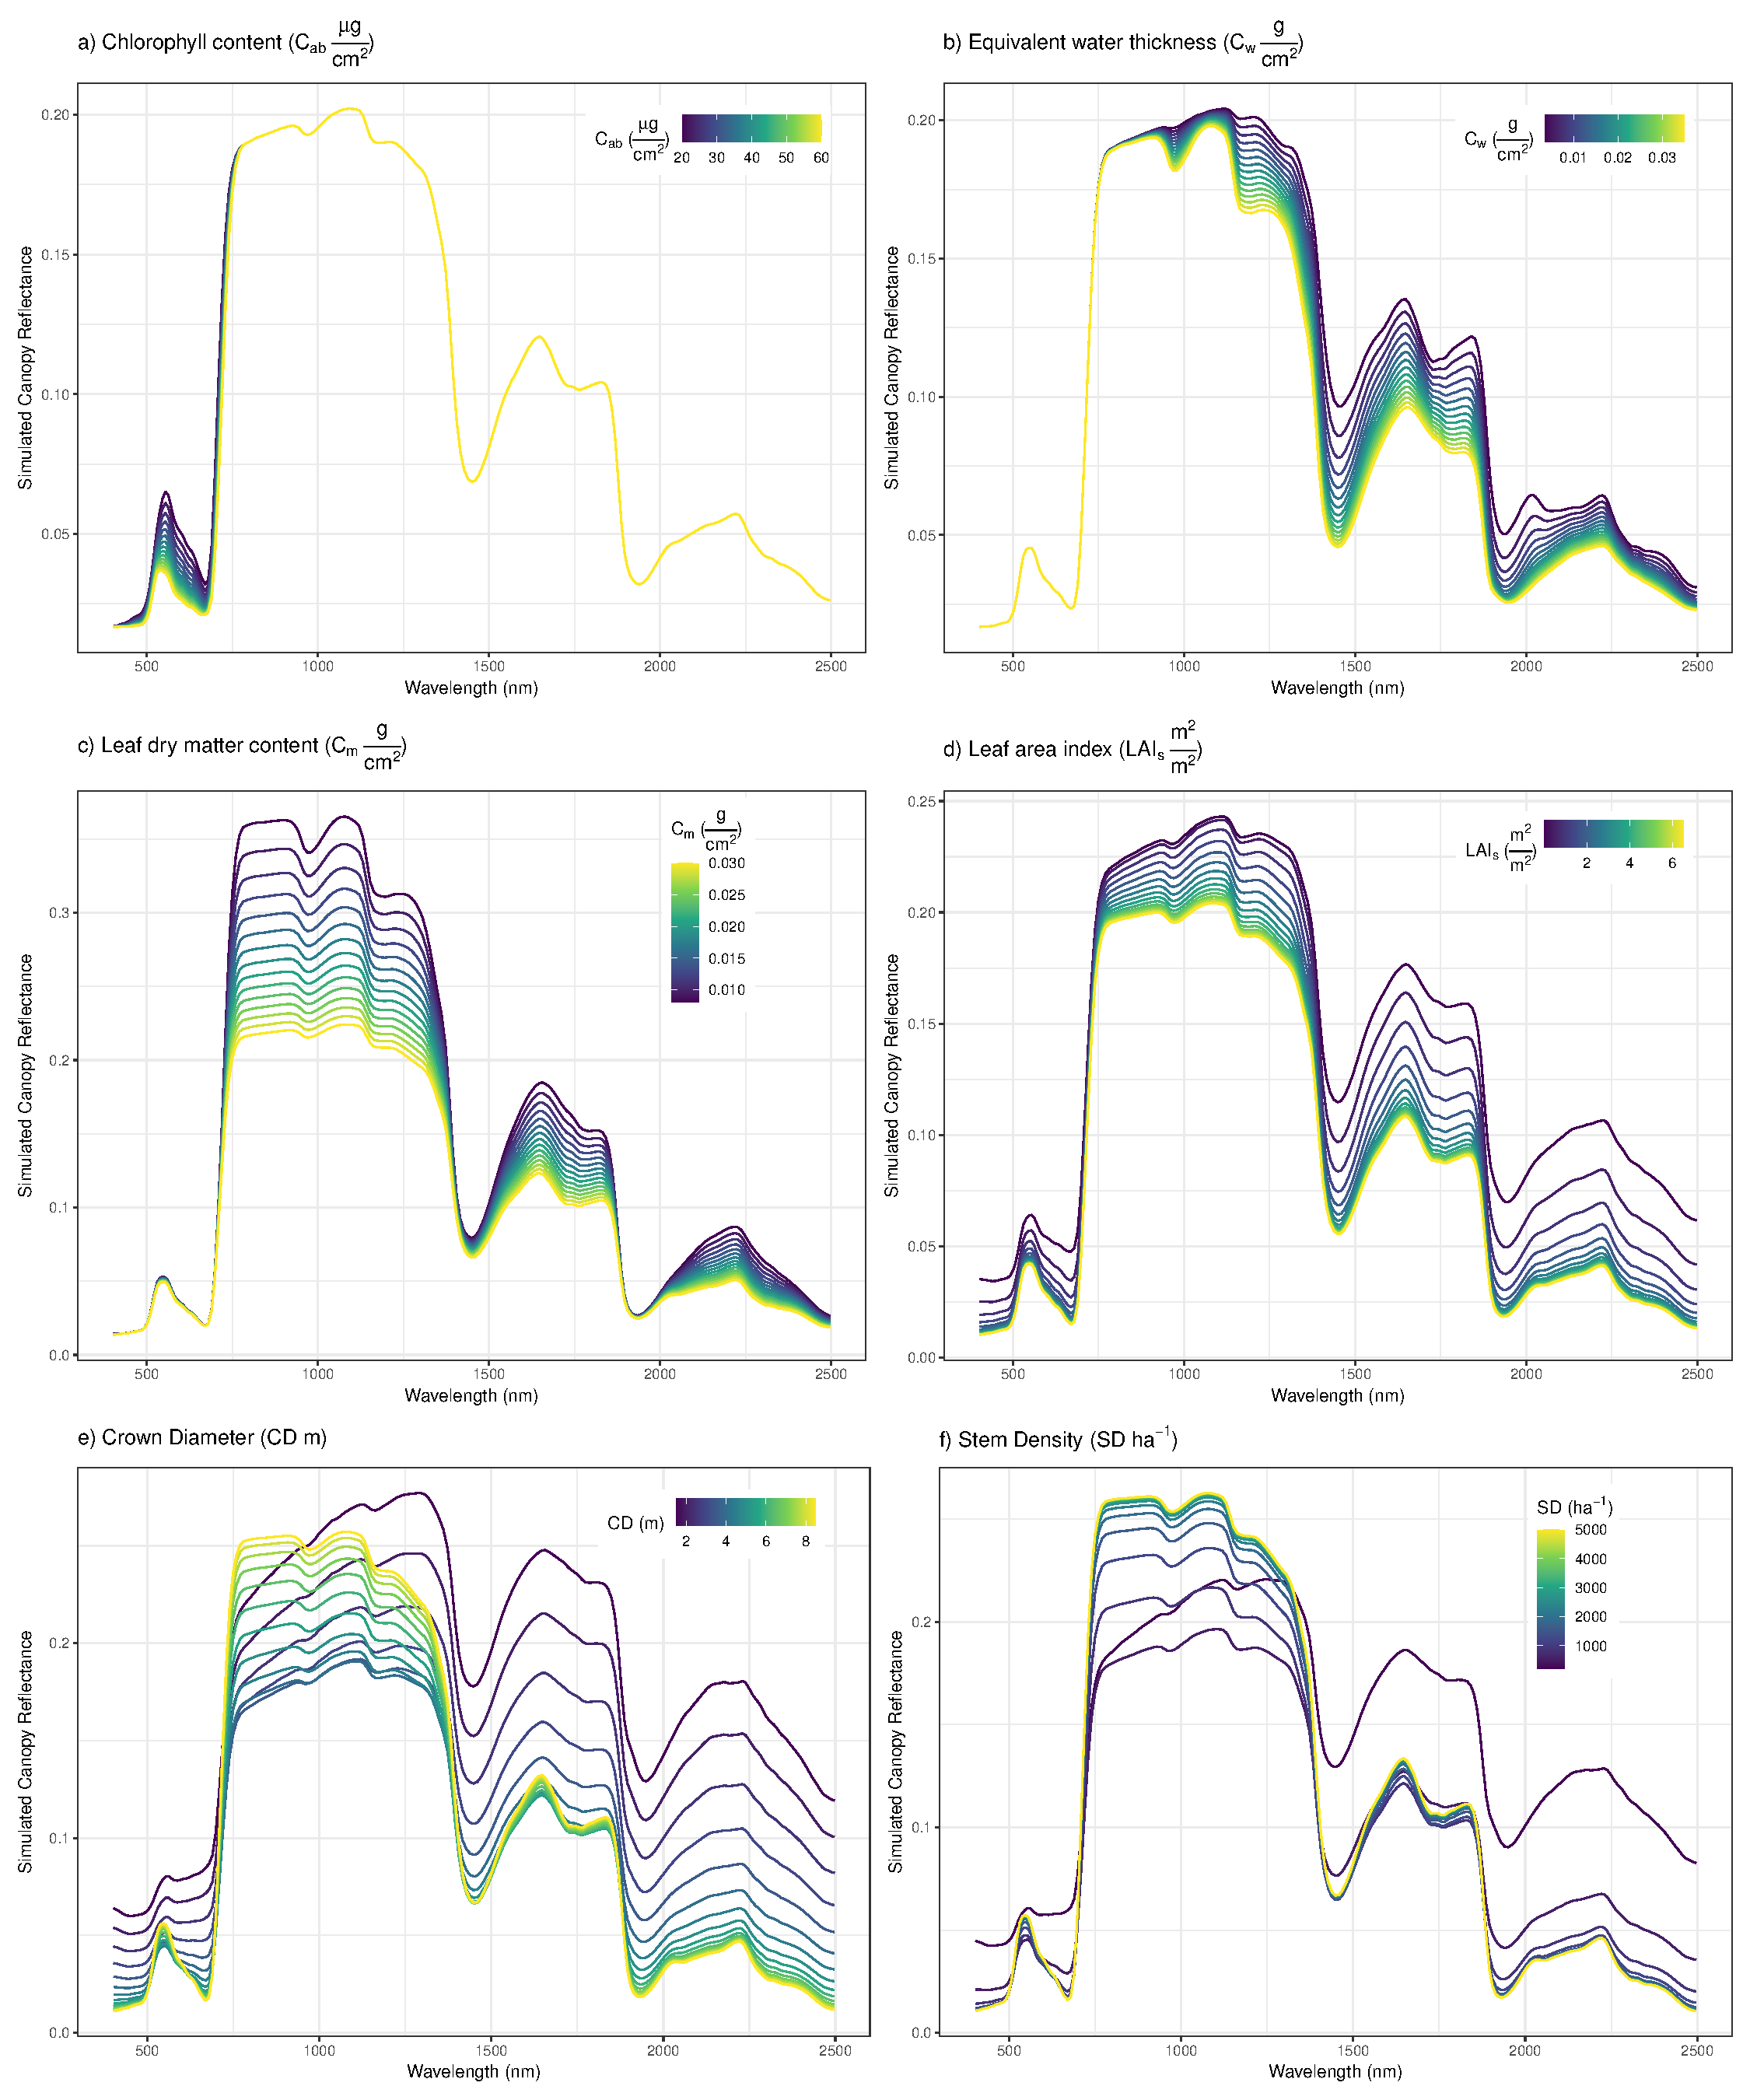
\includegraphics[height=0.8\textheight]{C:/Users/zavud/Desktop/msc_thesis/thesis/figures/sensitivity_results} 

}

\caption{Effects of varying the chosen parameters on the simulated spectra}\label{fig:fsens}
\end{figure}

\newpage

\hypertarget{rtm-simulation-inform-1}{%
\section{RTM simulation (INFORM)}\label{rtm-simulation-inform-1}}

Synthetic canopy reflectance data set were produced and stored in a LUT containing all 316,800 simulations. In this research, LUT was defined as a matrix. Each row of this matrix is a different simulated spectra and columns are simulated reflectance of wavelengths with the range of 400nm-2500nm with 1nm spectral resolution and 6 additional columns containing values of the corresponding variables \(C_{ab}\), \(C_{w}\), \(C_{m}\), \(LAI_{s}\), \(CD\) and \(SD\) that were used for each simulation. Hence the dimensions of the LUT matrix is 316,800 rows (number of simulations) by 2107 columns (2101 simulated ``bands'' + 6 INFORM variables):

\begingroup
\tiny

\[
\begin{bmatrix}
400nm_{1} & \dots & 2500nm_{1} & Cab_{1} & Cw_{1} & Cm_{1} & LAIs_{1} & CD_{1} & SD_{1}\\
400nm_{2} & \dots & 2500nm_{2} & Cab_{2} & Cw_{2} & Cm_{2} & LAIs_{2} & CD_{2} & SD_{2}\\
\ \vdots  &\ \vdots &\ \vdots &\ \vdots &\ \vdots &\ \vdots &\ \vdots &\ \vdots &\ \vdots\\
400nm_{316,800} & \dots & 2500nm_{316,800} & Cab_{316,800} & Cw_{316,800} & Cm_{316,800} & LAIs_{316,800} & CD_{316,800} & SD_{316,800}
\end{bmatrix}
\]
\endgroup

In this matrix, \(400nm_{n}\), \(\dots\), \(2500nm_{n}\) refer to the simulated reflectance for the corresponding wavelength in the simulation number \(n\). \(Cab_{n}\), \(Cw_{n}\), \(Cm_{n}\), \(LAIs_{n}\), \(CD_{n}\) and \(SD_{n}\) are values of the INFORM parameters that were used in the \(n\)th simulation.

\hypertarget{spectral-resampling-1}{%
\section{Spectral resampling}\label{spectral-resampling-1}}

The output of INFORM simulations were resampled to 231 PRISMA bands. The LUT matrix was used for spectral resampling and the resulting matrix has a dimension of 316,800 rows (number of simulations) by 237 columns (231 PRISMA image bands + 6 INFORM variables):

\begingroup
\tiny

\[
\begin{bmatrix}
Band1_{1} & \dots & Band231_{1} & Cab_{1} & Cw_{1} & Cm_{1} & LAIs_{1} & CD_{1} & SD_{1}\\
Band1_{2} & \dots & Band231_{2} & Cab_{2} & Cw_{2} & Cm_{2} & LAIs_{2} & CD_{2} & SD_{2}\\
\ \vdots  &\ \vdots &\ \vdots &\ \vdots &\ \vdots &\ \vdots &\ \vdots &\ \vdots &\ \vdots\\
Band1_{316,800} & \dots & Band231_{316,800} & Cab_{316,800} & Cw_{316,800} & Cm_{316,800} & LAIs_{316,800} & CD_{316,800} & SD_{316,800}
\end{bmatrix}
\]
\endgroup

In this matrix, \(Band1_{n}\), \(\dots\), \(Band231_{n}\) correspond to the simulated reflectance for the corresponding image band in the simulation number \(n\). \(Cab_{n}\), \(Cw_{n}\), \(Cm_{n}\), \(LAIs_{n}\), \(CD_{n}\) and \(SD_{n}\) refer to the values of the INFORM parameters that were used in the \(n\)th simulation.

\hypertarget{statistics-of-simulated-data-and-prisma-image-1}{%
\section{Statistics of simulated data and PRISMA image}\label{statistics-of-simulated-data-and-prisma-image-1}}

The Figure \ref{fig:statplots} shows statistical information (mean and mean \(\pm\) standard deviation) calculated from the LUT and PRISMA image:

\begin{figure}
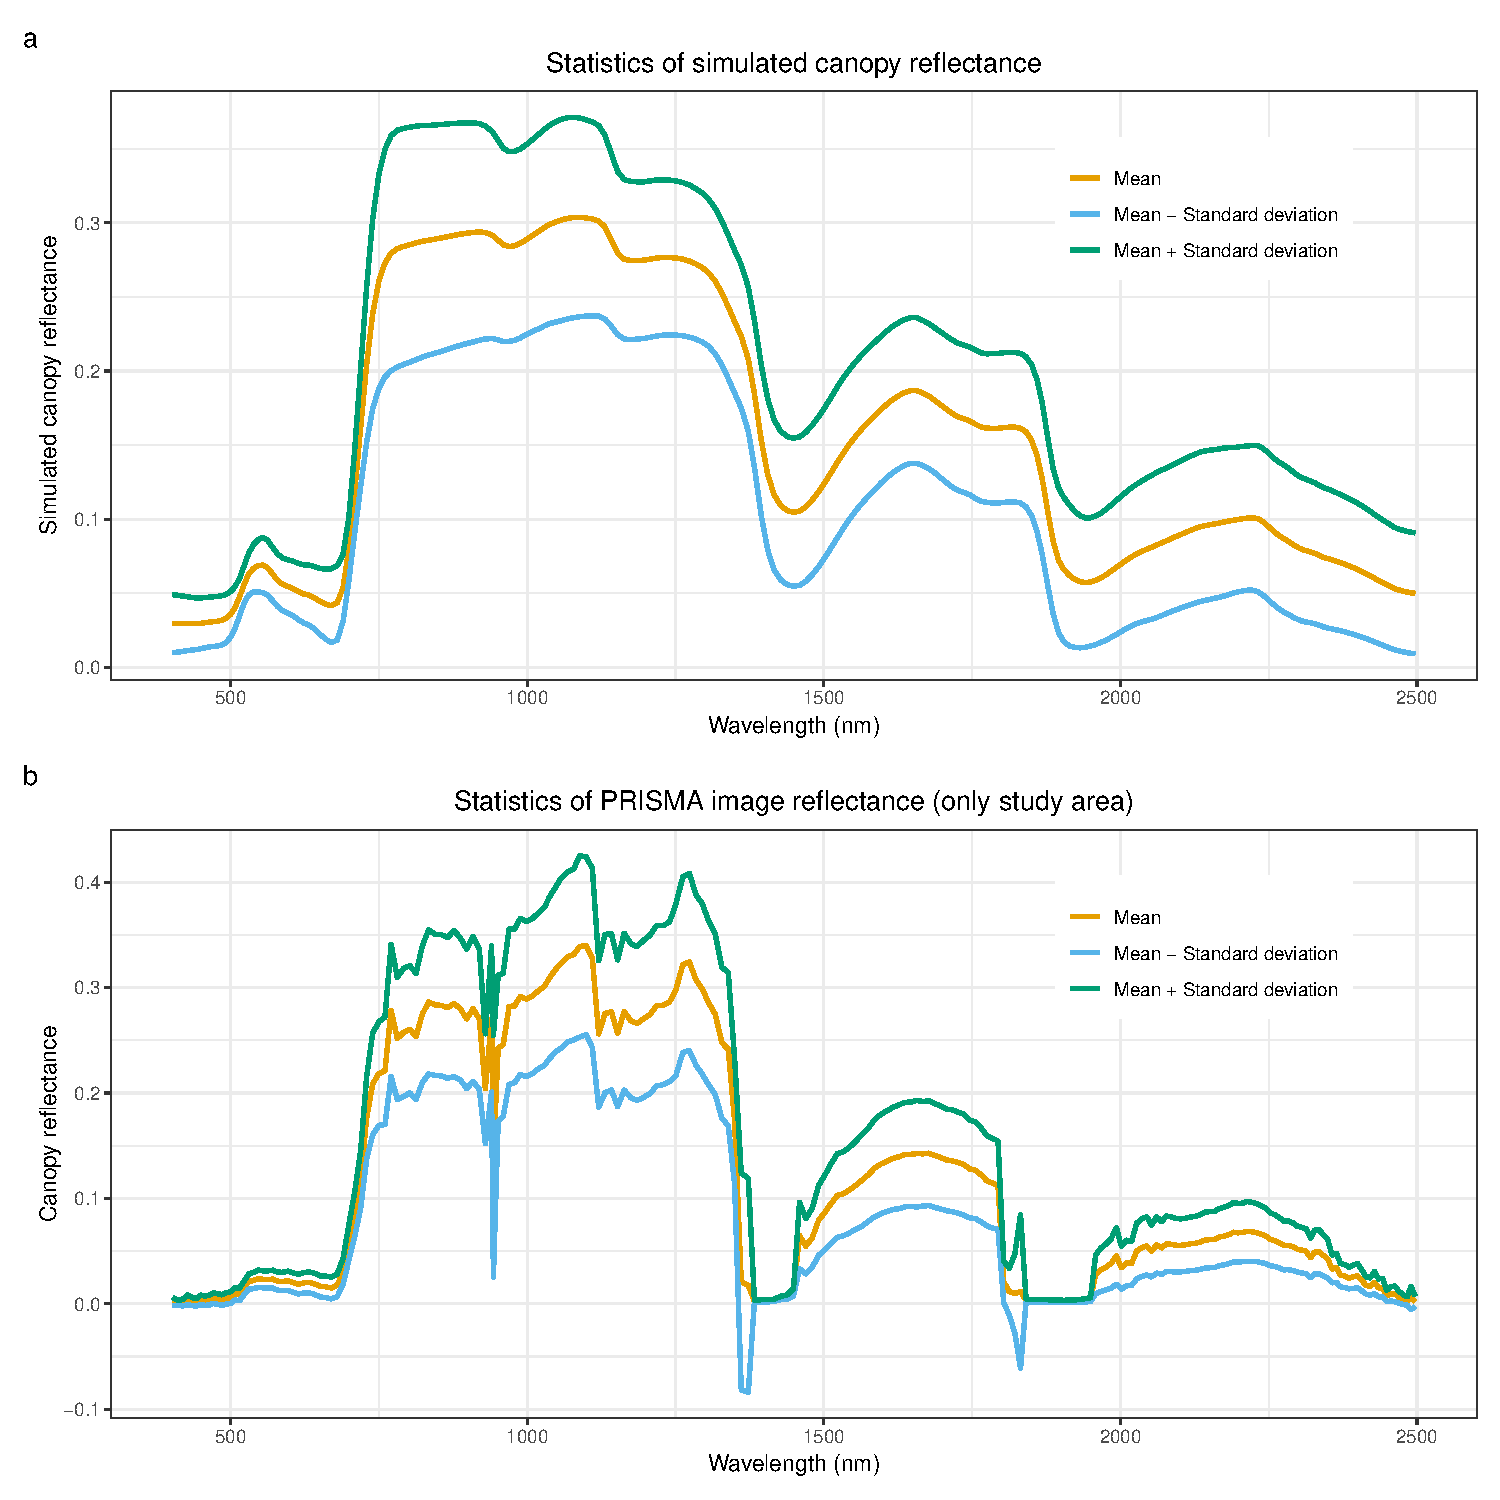
\includegraphics[width=0.9\linewidth]{C:/Users/zavud/Desktop/msc_thesis/thesis/figures/stats} \caption{Mean and mean $\pm$ standard deviation in the a) LUT and b) PRISMA image}\label{fig:statplots}
\end{figure}

Mean and standard deviation within the LUT are much smoother compared to mean and standard deviation within the PRISMA image spectra. This is due to the fact that INFORM model does not add noise during the simulation which can commonly exist in remote sensing images. There is a noticeable amount of noise in the PRISMA image spectra. Some of the noise in the image spectra could potentially be due to the fact that the PRISMA image contained cloud and shadow within the study area and although most of the cloud and shadow pixels were masked, the nearby pixels could still be affected.

The Figure \ref{fig:meancomparison} shows the difference between averaged reflectance within the simulated database (LUT) and PRISMA image.

\begin{figure}

{\centering 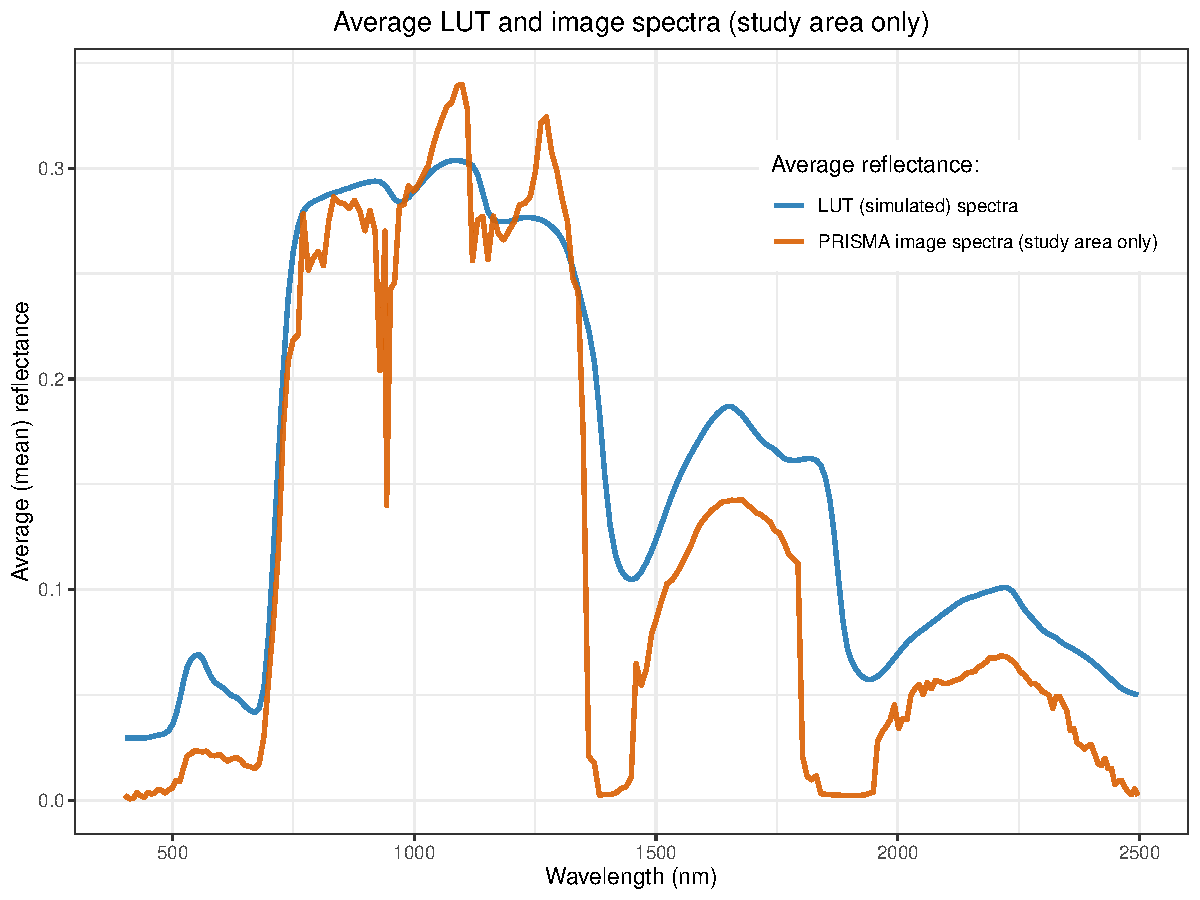
\includegraphics[width=0.8\linewidth]{C:/Users/zavud/Desktop/msc_thesis/thesis/figures/meancomparison_lut_vs_prisma} 

}

\caption{Difference between averaged LUT and PRISMA image reflectance}\label{fig:meancomparison}
\end{figure}

The LUT appears to have higher average reflectance within the visible spectra compared to the PRISMA image spectra. Differences within the water absorbtion bands can also be clearly seen. There is relatively good agreement within the NIR spectrum.

\newpage

\hypertarget{gaussian-noise-1}{%
\section{Gaussian noise}\label{gaussian-noise-1}}

The Figure \ref{fig:noise} shows the effect of adding 3\% Gaussian noise to the simulated data.

\begin{figure}
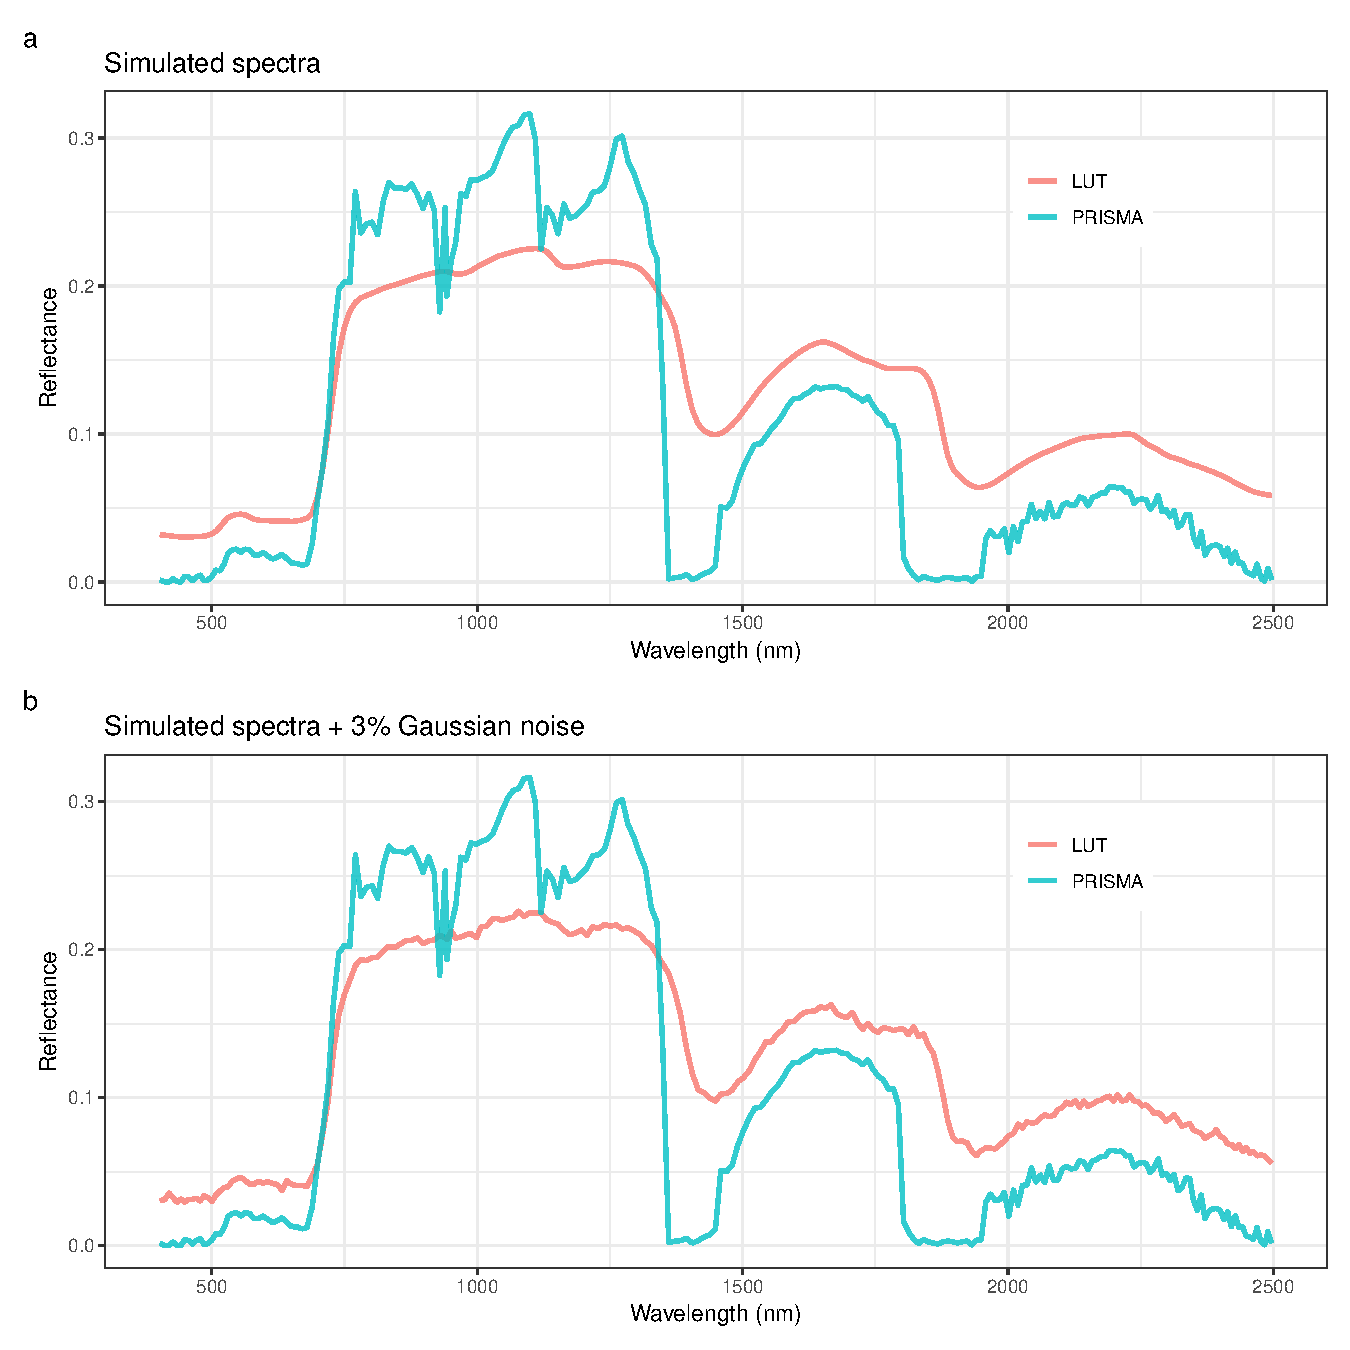
\includegraphics[width=0.9\linewidth]{C:/Users/zavud/Desktop/msc_thesis/thesis/figures/noise} \caption{Effect of adding $3\%$ Gaussian noise to the simulated spectra. The randomly chosen pixel from the PRISMA data was plotted to illustrate the noise found typically in the image}\label{fig:noise}
\end{figure}

The Figure \ref{fig:noise}.a shows a simulated spectra that seems perfectly smooth. However, after adding 3\% Gaussian noise, the simulated spectra is not as smooth anymore and contains random noise all over the whole spectra (Figure \ref{fig:noise}.b). This also makes the simulated spectra more similar to the pixel extracted from the PRISMA image.

\hypertarget{principal-component-analysis-pca-1}{%
\section{Principal Component Analysis (PCA)}\label{principal-component-analysis-pca-1}}

The result of PCA showed that most of the variation in the simulated data can be explained by much fewer variables (PCs):

\begin{figure}
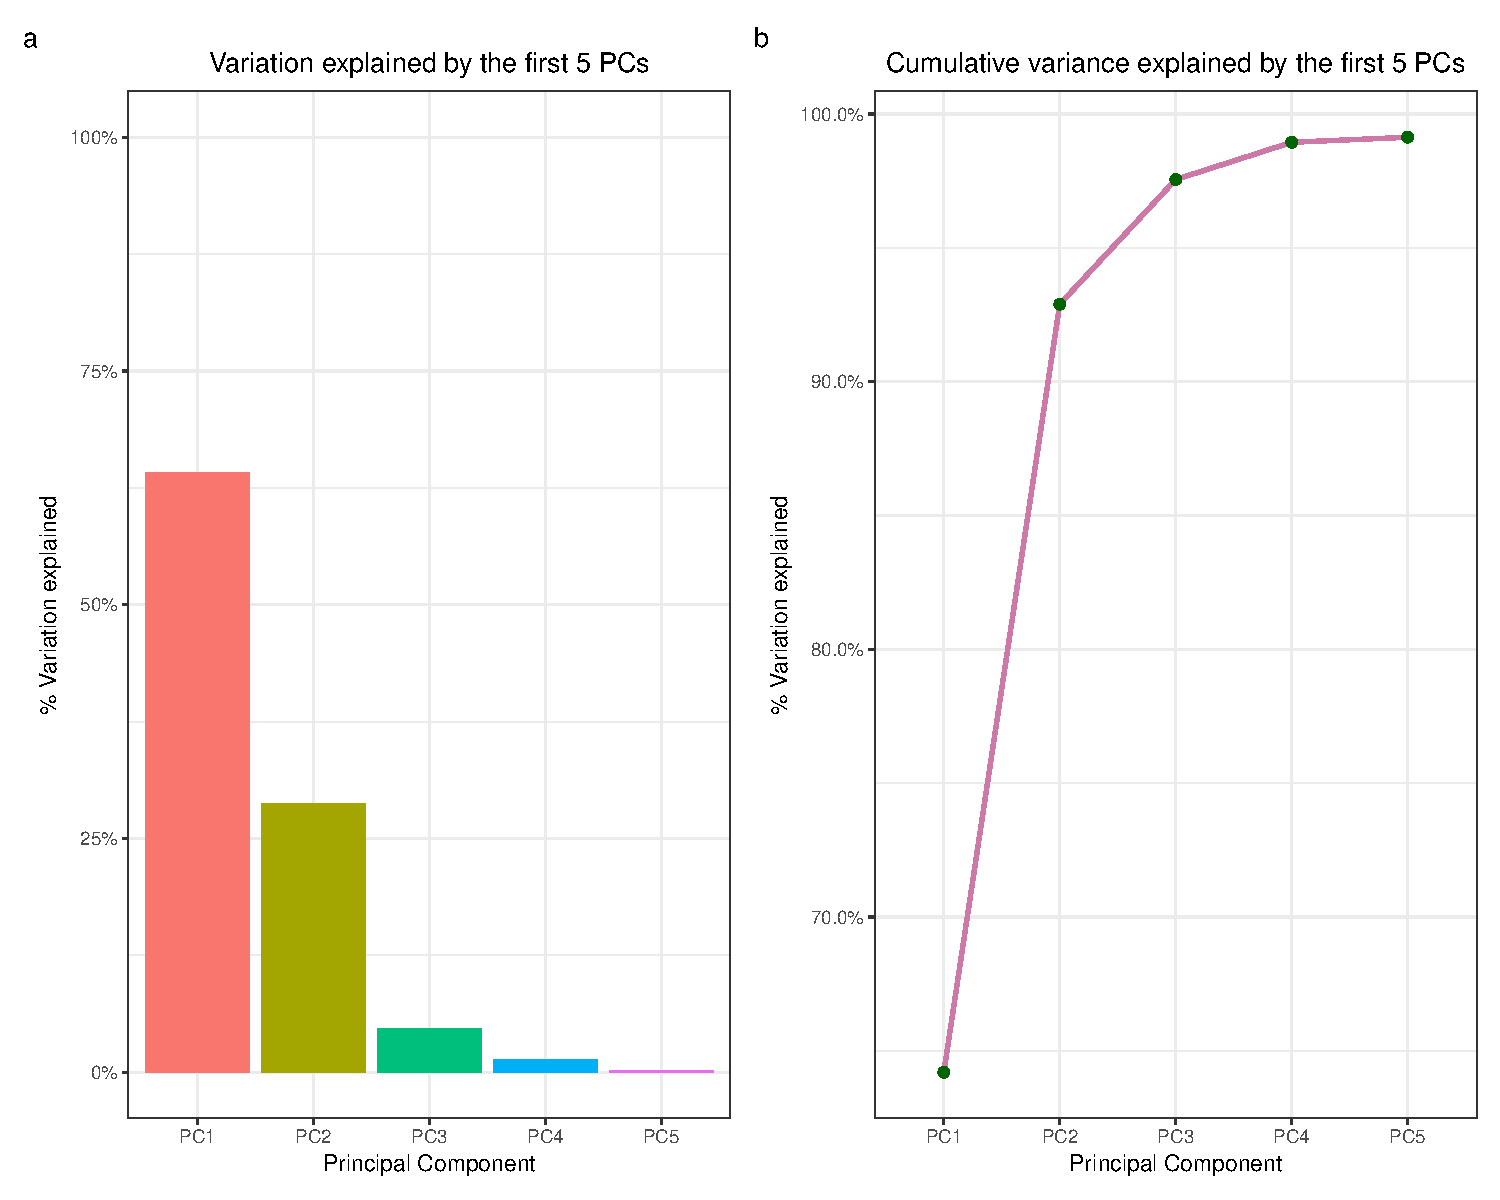
\includegraphics[width=0.9\linewidth]{C:/Users/zavud/Desktop/msc_thesis/thesis/figures/pca} \caption{Principal Component Analysis: a) Screeplot, b) Cumulative variance explained by the first 5 PCs}\label{fig:pca}
\end{figure}

The Figure \ref{fig:pca}.a shows the screeplot of the PCA result. The first PC explains the most of the variation and together with the next 4 PCs we can capture more than 99\% of the variation that is present in the original data (Figure \ref{fig:pca}.b). This, once again shows the multicollinearity problem with hyperspectral remote sensing data.


%%%%% REFERENCES

% JEM: Quote for the top of references (just like a chapter quote if you're using them).  Comment to skip.
% \begin{savequote}[8cm]
% The first kind of intellectual and artistic personality belongs to the hedgehogs, the second to the foxes \dots
%   \qauthor{--- Sir Isaiah Berlin \cite{berlin_hedgehog_2013}}
% \end{savequote}


\bibliography{references.bib}

\end{document}
